\subsubsection{steigen und sinken}

Es gibt verschieden Arten von Funktionen:\\
\begin{itemize}
    \item \textcolor{red}{Streng monoton steigend $f'(x)>0$}
    \item \textcolor{violet}{Konstant $f'(x)=0$}
    \item \textcolor{blue}{Streng monoton fallend $f'(x)<0$ }
\end{itemize}

\hfill \break

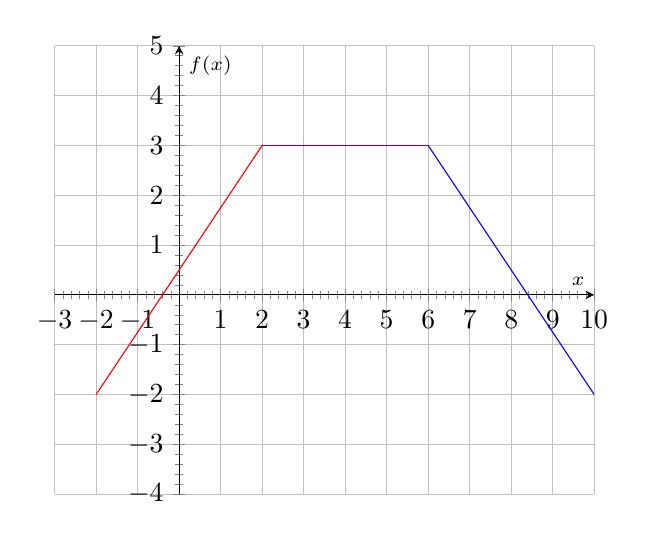
\begin{tikzpicture}[scale=1.0]
    \begin{axis}%
        [
            grid=major,
            xtick={-7,-6,...,11},
            minor x tick num=4, % 4 minor ticks => 5 subintervals
            xmin=-3,
            xmax=10,
            xlabel={\scriptsize $x$},
            axis x line=middle,
            ytick={-6,-5,...,6},
            minor y tick num=4,  % 4 minor ticks => 5 subintervals
            ymin=-4,
            ymax=5,
            ylabel={\scriptsize $f(x)$},
            axis y line=middle,
            no markers,
            samples=100,
            domain=-6:6,
        ]
        \draw[red] (-2,-2) -- (2,3);
        \draw[violet] (2,3) -- (6,3);
        \draw[blue] (6,3) -- (10,-2);
    \end{axis}
\end{tikzpicture}